\documentclass[english]{SPFShortReport}
\usepackage{subfigure}
\usepackage{spfFigures}
\usepackage{longtable}
\usepackage{url}
\usepackage{gensymb}
\usepackage[yyyymmdd,hhmmss]{datetime}
\reportName{Python calculation for heat pump SIN-18TU}
\reportSubName{Parametric Heat Pump calculation} 
\reportDate{\today \hspace{0.1cm} at: \currenttime \hspace{0.1cm} h} 
\author{Dani Carbonell}
\address{dani.carbonell@solarenergy.ch}
\begin{document}
\begin{table}[!ht]
\begin{small}
\caption{Fitted coefficients for the heat pump.}
\begin{center}
\resizebox{12cm}{!} 
{
\begin{tabular}{l | c c } 
\hline
\hline
Coefficient &Description & \\ 
 & &$[kW]$\\ 
\hline
$PQ_{1}$ & \emph{$1^{st}$ condenser polynomial coefficient}  & 1.6031e+01    \\ 
$PQ_{2}$ & \emph{$2^{st}$ condenser polynomial coefficient}  & 1.6862e+02    \\ 
$PQ_{3}$ & \emph{$3^{st}$ condenser polynomial coefficient}  & 4.5006e+01    \\ 
$PQ_{4}$ & \emph{$4^{st}$ condenser polynomial coefficient}  & -3.0845e+02    \\ 
$PQ_{5}$ & \emph{$5^{st}$ condenser polynomial coefficient}  & 2.7295e+02    \\ 
$PQ_{6}$ & \emph{$6^{st}$ condenser polynomial coefficient}  & -1.9880e+02    \\ 
\hline
$PCOP_{1}$ & \emph{$1^{st}$ COP polynomial coefficient}  & 6.0450e+00    \\ 
$PCOP_{2}$ & \emph{$2^{st}$ COP polynomial coefficient}  & 5.1596e+01    \\ 
$PCOP_{3}$ & \emph{$3^{st}$ COP polynomial coefficient}  & 4.8630e-01    \\ 
$PCOP_{4}$ & \emph{$4^{st}$ COP polynomial coefficient}  & -1.9286e+02    \\ 
$PCOP_{5}$ & \emph{$5^{st}$ COP polynomial coefficient}  & -2.0545e+01    \\ 
$PCOP_{6}$ & \emph{$6^{st}$ COP polynomial coefficient}  & -8.4732e+01    \\ 
\hline
$\dot m_{cond}$ & 3000.00 $[kg/h]$\\ 
$\dot m_{evap}$ & 3000.00 $[kg/h]$\\ 
\hline
$COP_{nom}$ (B0W35)& 4.68 \\ 
$Q_{c,nom}$ (B0W35)& 17.54 kW\\ 
$COP_{nom}$ (B2W35)& 4.88 \\ 
$Q_{c,nom}$ (B2W35)& 18.43 kW\\ 
$COP_{nom}$ (B10W35)& 5.70 \\ 
$Q_{c,nom}$ (B10W35)& 22.22 kW\\ 
\hline
\hline
\end{tabular}
}
\label{CoefTable}
\end{center}
\end{small}
\end{table}
\begin{table}[!ht]
\begin{small}
\caption{Predicting results of the heat pump.}
\begin{center}
\resizebox{12cm}{!} 
{
\begin{tabular}{l | c c c c c c c c c c c } 
\hline
\hline
$T_{evap,in}$ &$T_{evap,out}$ &$T_{cond,in}$ &$T_{cond,out}$ &$COP$ &$Q_{cond}$ &$Q_{evap}$ &$W_{comp}$ &$\dot m_{cond}$ &$\dot m_{evap}$ &$\Delta T_{evap}$ &$\Delta T_{cond}$ \\ 
$^oC$ &$^oC$ &$^oC$ &$^oC$ &$[-]$ &$[kW]$ &$[kW]$ &$[kW]$ &kg/h &kg/h &K &K\\ 
\hline
-7.00 & -10.45 & 25.86 & 30.00 & 4.17 & 14.45 & 10.99 & 3.47 & 3000 & 3000 & 3.5 & 4.1\\ 
-7.00 & -10.39 & 34.54 & 38.75 & 3.75 & 14.72 & 10.79 & 3.93 & 3000 & 3000 & 3.4 & 4.2\\ 
-7.00 & -10.14 & 43.32 & 47.50 & 3.15 & 14.61 & 9.97 & 4.64 & 3000 & 3000 & 3.1 & 4.2\\ 
-7.00 & -9.57 & 52.21 & 56.25 & 2.38 & 14.12 & 8.19 & 5.94 & 3000 & 3000 & 2.6 & 4.0\\ 
-7.00 & -8.25 & 61.19 & 65.00 & 1.42 & 13.31 & 3.96 & 9.35 & 3000 & 3000 & 1.2 & 3.8\\ 
-4.00 & -7.84 & 25.50 & 30.00 & 4.52 & 15.70 & 12.23 & 3.48 & 3000 & 3000 & 3.8 & 4.5\\ 
-4.00 & -7.76 & 34.20 & 38.75 & 4.03 & 15.88 & 11.94 & 3.94 & 3000 & 3000 & 3.8 & 4.5\\ 
-4.00 & -7.47 & 43.01 & 47.50 & 3.38 & 15.68 & 11.04 & 4.64 & 3000 & 3000 & 3.5 & 4.5\\ 
-4.00 & -6.88 & 51.92 & 56.25 & 2.54 & 15.11 & 9.17 & 5.94 & 3000 & 3000 & 2.9 & 4.3\\ 
-4.00 & -5.54 & 60.93 & 65.00 & 1.52 & 14.22 & 4.89 & 9.33 & 3000 & 3000 & 1.5 & 4.1\\ 
-1.00 & -5.25 & 25.13 & 30.00 & 4.86 & 17.01 & 13.51 & 3.50 & 3000 & 3000 & 4.2 & 4.9\\ 
-1.00 & -5.13 & 33.85 & 38.75 & 4.32 & 17.10 & 13.14 & 3.96 & 3000 & 3000 & 4.1 & 4.9\\ 
-1.00 & -4.82 & 42.68 & 47.50 & 3.60 & 16.82 & 12.15 & 4.67 & 3000 & 3000 & 3.8 & 4.8\\ 
-1.00 & -4.21 & 51.62 & 56.25 & 2.71 & 16.16 & 10.19 & 5.97 & 3000 & 3000 & 3.2 & 4.6\\ 
-1.00 & -2.83 & 60.65 & 65.00 & 1.62 & 15.19 & 5.83 & 9.36 & 3000 & 3000 & 1.8 & 4.4\\ 
2.00 & -2.67 & 24.74 & 30.00 & 5.20 & 18.38 & 14.84 & 3.53 & 3000 & 3000 & 4.7 & 5.3\\ 
2.00 & -2.52 & 33.49 & 38.75 & 4.60 & 18.38 & 14.39 & 3.99 & 3000 & 3000 & 4.5 & 5.3\\ 
2.00 & -2.18 & 42.34 & 47.50 & 3.83 & 18.02 & 13.31 & 4.71 & 3000 & 3000 & 4.2 & 5.2\\ 
2.00 & -1.54 & 51.30 & 56.25 & 2.87 & 17.28 & 11.25 & 6.02 & 3000 & 3000 & 3.5 & 4.9\\ 
2.00 & -0.14 & 60.35 & 65.00 & 1.72 & 16.23 & 6.79 & 9.43 & 3000 & 3000 & 2.1 & 4.6\\ 
5.00 & -0.10 & 24.33 & 30.00 & 5.54 & 19.80 & 16.23 & 3.57 & 3000 & 3000 & 5.1 & 5.7\\ 
5.00 & 0.07 & 33.10 & 38.75 & 4.88 & 19.72 & 15.68 & 4.04 & 3000 & 3000 & 4.9 & 5.6\\ 
5.00 & 0.44 & 41.98 & 47.50 & 4.05 & 19.27 & 14.51 & 4.76 & 3000 & 3000 & 4.6 & 5.5\\ 
5.00 & 1.11 & 50.97 & 56.25 & 3.03 & 18.45 & 12.36 & 6.09 & 3000 & 3000 & 3.9 & 5.3\\ 
5.00 & 2.55 & 60.04 & 65.00 & 1.82 & 17.32 & 7.79 & 9.54 & 3000 & 3000 & 2.4 & 5.0\\ 
8.00 & 2.45 & 23.91 & 30.00 & 5.88 & 21.28 & 17.66 & 3.62 & 3000 & 3000 & 5.6 & 6.1\\ 
8.00 & 2.64 & 32.70 & 38.75 & 5.17 & 21.12 & 17.03 & 4.09 & 3000 & 3000 & 5.4 & 6.0\\ 
8.00 & 3.04 & 41.60 & 47.50 & 4.27 & 20.59 & 15.76 & 4.82 & 3000 & 3000 & 5.0 & 5.9\\ 
8.00 & 3.75 & 50.61 & 56.25 & 3.19 & 19.68 & 13.51 & 6.18 & 3000 & 3000 & 4.2 & 5.6\\ 
8.00 & 5.23 & 59.71 & 65.00 & 1.91 & 18.48 & 8.82 & 9.67 & 3000 & 3000 & 2.8 & 5.3\\ 
11.00 & 4.98 & 23.47 & 30.00 & 6.22 & 22.81 & 19.15 & 3.67 & 3000 & 3000 & 6.0 & 6.5\\ 
11.00 & 5.21 & 32.28 & 38.75 & 5.44 & 22.57 & 18.43 & 4.15 & 3000 & 3000 & 5.8 & 6.5\\ 
11.00 & 5.63 & 41.21 & 47.50 & 4.49 & 21.96 & 17.07 & 4.89 & 3000 & 3000 & 5.4 & 6.3\\ 
11.00 & 6.38 & 50.24 & 56.25 & 3.34 & 20.98 & 14.70 & 6.27 & 3000 & 3000 & 4.6 & 6.0\\ 
11.00 & 7.89 & 59.36 & 65.00 & 2.01 & 19.70 & 9.88 & 9.82 & 3000 & 3000 & 3.1 & 5.6\\ 
14.00 & 7.50 & 23.01 & 30.00 & 6.56 & 24.41 & 20.68 & 3.72 & 3000 & 3000 & 6.5 & 7.0\\ 
14.00 & 7.75 & 31.85 & 38.75 & 5.72 & 24.09 & 19.88 & 4.21 & 3000 & 3000 & 6.3 & 6.9\\ 
14.00 & 8.21 & 40.80 & 47.50 & 4.71 & 23.39 & 18.42 & 4.97 & 3000 & 3000 & 5.8 & 6.7\\ 
14.00 & 8.98 & 49.85 & 56.25 & 3.50 & 22.33 & 15.95 & 6.38 & 3000 & 3000 & 5.0 & 6.4\\ 
14.00 & 10.54 & 58.99 & 65.00 & 2.10 & 20.99 & 11.00 & 9.99 & 3000 & 3000 & 3.5 & 6.0\\ 
17.00 & 10.00 & 22.54 & 30.00 & 6.89 & 26.05 & 22.27 & 3.78 & 3000 & 3000 & 7.0 & 7.5\\ 
17.00 & 10.28 & 31.40 & 38.75 & 6.00 & 25.65 & 21.38 & 4.28 & 3000 & 3000 & 6.7 & 7.3\\ 
17.00 & 10.77 & 40.37 & 47.50 & 4.92 & 24.88 & 19.83 & 5.05 & 3000 & 3000 & 6.2 & 7.1\\ 
17.00 & 11.58 & 49.45 & 56.25 & 3.66 & 23.74 & 17.25 & 6.49 & 3000 & 3000 & 5.4 & 6.8\\ 
17.00 & 13.18 & 58.61 & 65.00 & 2.19 & 22.33 & 12.15 & 10.18 & 3000 & 3000 & 3.8 & 6.4\\ 
20.00 & 12.48 & 22.05 & 30.00 & 7.22 & 27.76 & 23.91 & 3.84 & 3000 & 3000 & 7.5 & 7.9\\ 
20.00 & 12.79 & 30.94 & 38.75 & 6.27 & 27.28 & 22.93 & 4.35 & 3000 & 3000 & 7.2 & 7.8\\ 
20.00 & 13.31 & 39.93 & 47.50 & 5.14 & 26.43 & 21.29 & 5.14 & 3000 & 3000 & 6.7 & 7.6\\ 
20.00 & 14.15 & 49.03 & 56.25 & 3.81 & 25.21 & 18.60 & 6.61 & 3000 & 3000 & 5.8 & 7.2\\ 
20.00 & 15.80 & 58.20 & 65.00 & 2.29 & 23.73 & 13.36 & 10.37 & 3000 & 3000 & 4.2 & 6.8\\ 
\hline
\hline
\end{tabular}
}
\label{ResultsTable}
\end{center}
\end{small}
\end{table}
\begin{figure}[!ht]
\begin{center}
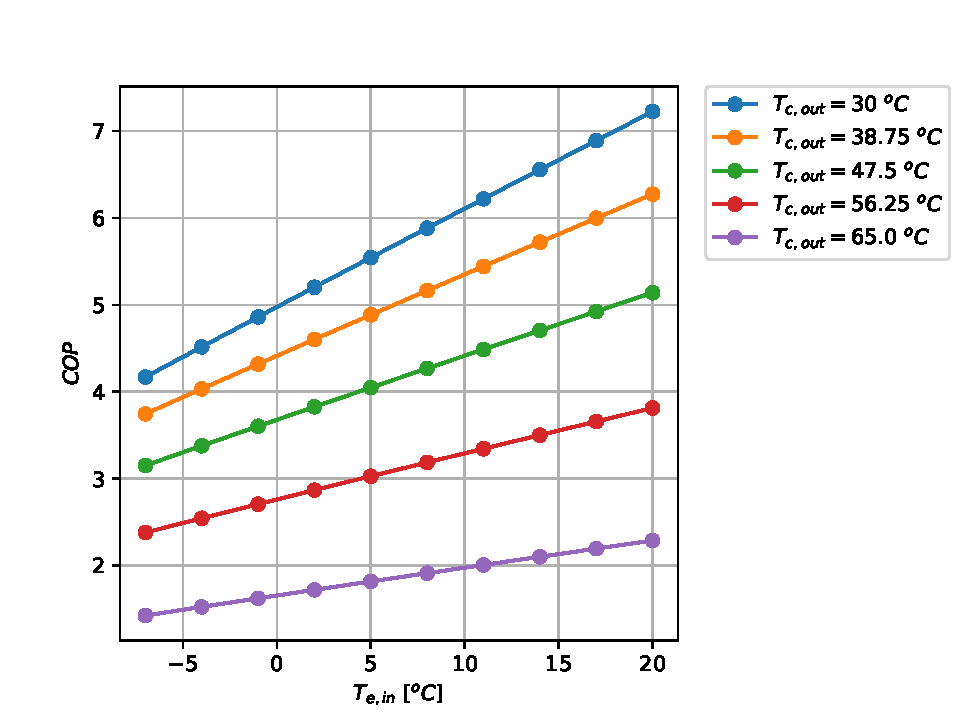
\includegraphics[width=1\textwidth]{C:/Daten/spfPackages/GIT/spfTrnsysFiles/HeatPump/BrineToWater/Walter Meier/SIN-18TU/SIN-18TU-Cop.pdf}
\caption{COP Results for the heat pump at the selected points}
\label{COPFig}
\end{center}
\end{figure}
\begin{figure}[!ht]
\begin{center}
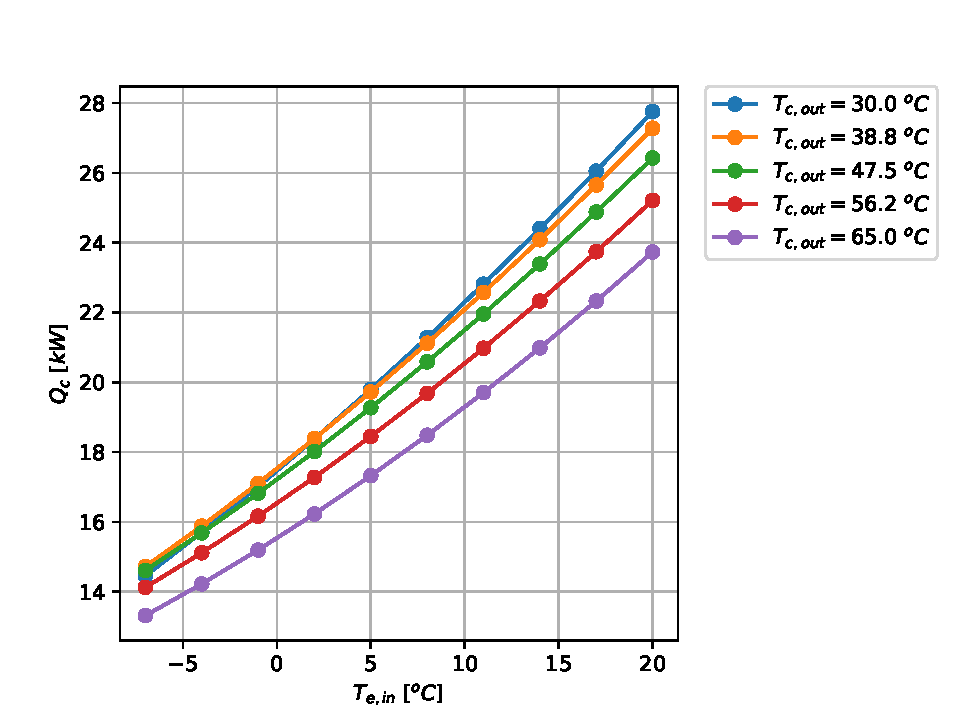
\includegraphics[width=1\textwidth]{C:/Daten/spfPackages/GIT/spfTrnsysFiles/HeatPump/BrineToWater/Walter Meier/SIN-18TU/SIN-18TU-Qc.pdf}
\caption{$Q_c$ Results for the heat pump at the selected points}
\label{QcFig}
\end{center}
\end{figure}
\end{document}
